\section{How Task Complexity Shifts The Bottleneck To Recovery Cost}
\label{sec:recovery-ablation}

Sections~\ref{sec:po-identification} and~\ref{sec:memory-structure} established that under PO, memory existence matters more than memory structure for the current task suite. This section shows that as task complexity increases from single-goal to multi-stage manipulation, the bottleneck shifts further: beyond retaining goal information, the system must also manage execution and recovery within a finite step budget.

\subsection{The Complexity Pivot}

The three solvable tasks differ in structural complexity. \task{reach-v3} and \task{push-v3} require the controller to reach a goal position and, in the case of \task{push-v3}, apply a force---but the action sequence is essentially single-stage. \task{pick-place-v3} is different: it requires a multi-stage grasp sequence (approach, descend, grasp, lift, move, release), where each stage depends on the successful completion of the prior one. This structural difference creates a qualitative shift in the system's failure modes.

In single-stage tasks, the dominant failure mode is information loss: without persistent memory, the controller cannot maintain goal-directed behavior. In multi-stage tasks, a second failure mode emerges: even with persistent memory, a naive recovery mechanism can consume the finite episode budget by repeatedly re-traversing already-completed stages.

\subsection{Retry=0 vs.\ Retry=3}

\begin{figure}[t]
  \centering
  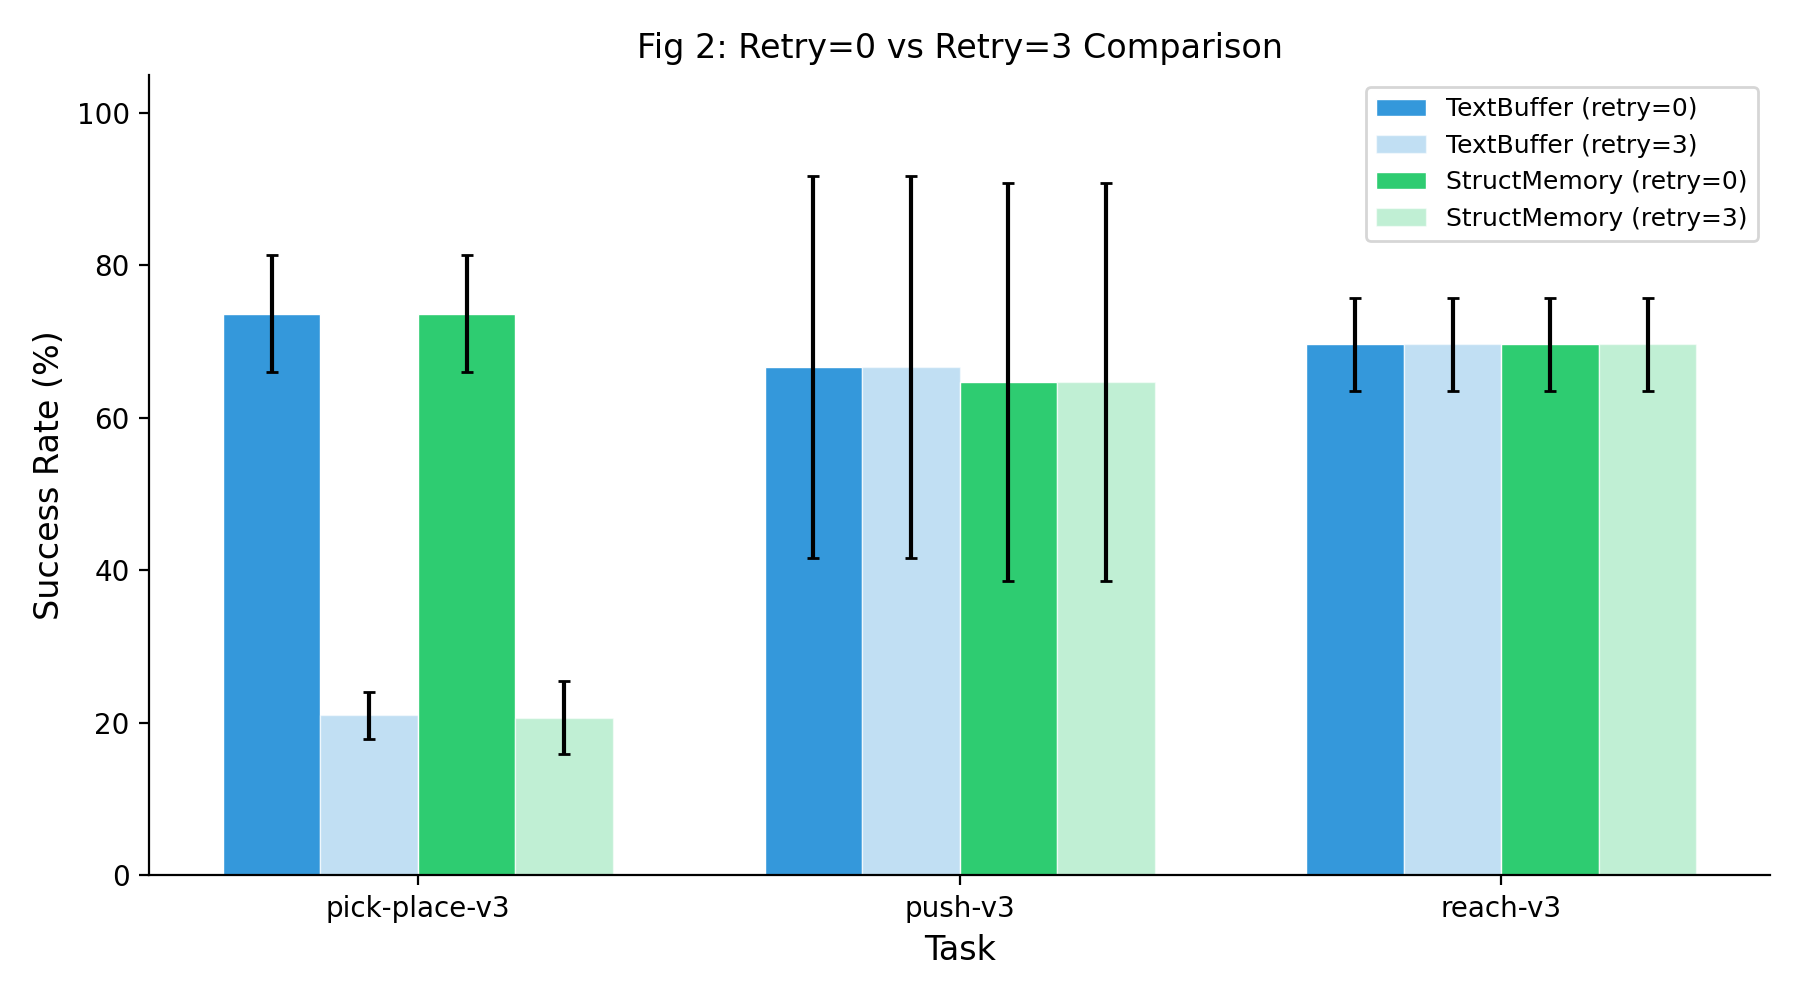
\includegraphics[width=0.92\linewidth]{figures/fig2_retry_comparison.png}
  \caption{Effect of retry mechanism on \task{pick-place-v3}. Disabling retry (\texttt{retry=0}) raises success from 21.0\% to 73.7\%, a +52.7pp gain. No comparable effect appears on simpler tasks.}
  \label{fig:retry-ablation}
\end{figure}

\begin{table}[htbp]
\centering
\caption{Ablation study results (success rate \%). P3A: no goal flashing; P3B: no retry; P3C: no XY perturbation.}
\label{tab:ablation}
\begin{tabular}{llccc}
\toprule
Ablation & Task & NoMemory & TextBuffer & StructMemory \\
\midrule
No Flash & pick-place-v3 & 0.0 & 18.9 & 21.1 \\
No Flash & push-v3 & 0.0 & 71.1 & 70.0 \\
No Flash & reach-v3 & 0.0 & 65.0 & 65.0 \\
\midrule
No Retry & door-open-v3 & — & 0.0 & 0.0 \\
No Retry & pick-place-v3 & — & 71.7 & 71.7 \\
\midrule
No Perturb & door-open-v3 & — & — & 0.0 \\
No Perturb & pick-place-v3 & — & — & 20.6 \\
\bottomrule
\end{tabular}
\end{table}

As shown in Table~\ref{tab:ablation} and Figure~\ref{fig:retry-ablation}, disabling retry substantially improves \task{pick-place-v3}. Under \texttt{retry=0}, both \task{TextBuffer} and \task{StructMemory} reach $73.7\%$. Under the older \texttt{retry=3} configuration, the same task reaches only $21.0\%$ for \task{TextBuffer} and $20.7\%$ for \task{StructMemory}---a gap of $+52.7$ and $+53.0$ percentage points, respectively.

The effect is sharply task-specific. The retry comparison produces no comparable shift on \task{reach-v3}, \task{push-v3}, or \task{door-open-v3}. This pattern confirms that the problem lies in how rollback interacts with the sequential structure of \task{pick-place-v3}, rather than in a generic benefit of disabling retry everywhere.

\subsection{Mechanism: Retry Budget Consumption}

\begin{figure}[t]
  \centering
  \includegraphics[width=0.92\linewidth]{figures/fig_retry_budget_consumption.pdf}
  \caption{Retry budget consumption on \task{pick-place-v3} (\texttt{retry=3}). Each rollback event forces the controller to re-traverse the descend and grasp stages, which together account for over 70\% of step consumption. The 390 rollback events across episodes illustrate how recovery cost accumulates under a finite horizon.}
  \label{fig:retry-budget}
\end{figure}

Figure~\ref{fig:retry-budget} visualizes the mechanism behind the retry penalty. Under \texttt{retry=3}, the controller accumulates 390 rollback events across episodes. Each rollback returns the controller to an earlier stage of the grasp sequence, forcing it to re-execute the descend and grasp phases---which together account for over 70\% of the step consumption per episode. Under a 200-step budget, this repeated re-traversal leaves insufficient steps for the later lift, move, and release stages that are necessary for task completion.

The core problem is opportunity cost. The retry mechanism is designed to recover from local failures by re-approaching the grasp, but each rollback consumes steps that could have been spent progressing toward task completion. In a multi-stage task where the early stages (descend, grasp) are the most failure-prone, the controller can become trapped in a cycle of re-executing the same expensive stages without ever reaching the later ones.

\subsection{Conclusion}

In multi-stage manipulation tasks, the bottleneck shifts from information availability to recovery cost. When rollback is expensive relative to the episode budget, a naive retry mechanism becomes a new source of failure rather than a corrective strategy. This finding extends the paper's layered view: the first bottleneck (information loss) is addressed by persistent memory; the second bottleneck (recovery cost) requires explicit budget-aware recovery design. The two bottlenecks are not independent---they interact through the finite horizon constraint that binds both memory retention and execution planning.
